\documentclass[11pt,a4paper]{article}
\usepackage{ifpdf}
\usepackage[utf8]{inputenc}
\usepackage[francais]{babel}
\usepackage[T1]{fontenc}
\usepackage[nottoc, notlof, notlot]{tocbibind}
\usepackage{graphicx} 
\parindent 1.0cm

\title{Projet d'Intelligence Artificielle : L'ATARI-GO}
\author{Anthony \textsc{Caillaud} Manoël \textsc{Fortun}}
\date{\today}
\ifpdf
\pdfinfo {
	/Author (Anthony Caillaud Manoël Fortun)
	/Title (Projet d'Intelligence Artificielle : L'ATARI-GO)
	/Subject (Projet d'Intelligence Artificielle : L'ATARI-GO)
	/Keywords ()
	/CreationDate (D:20100329212218)
}
\fi

\begin{document}
	\maketitle
	\clearpage
	\tableofcontents
	\clearpage

\section{Introduction}
Ce dossier a pour but de rendre compte du travail effectué dans le cadre des
Travaux Pratiques du module d'Intelligence Artificielle.

 L'objectif du projet est de réaliser un programme permettant de jouer au jeu
 de l'Atari-go. Notre travail s'est divisé en deux grandes parties : 
 la mise en place d'une partie interface et la mise en place de l'intelligence 
 artificielle.

Dans un premier temps, nous allons présenter le projet et ses
différents objectifs. Ensuite, nous allons vous exposer les
différentes parties du développement. Enfin, nous conclurons par les
difficultés rencontrées et l'état du projet final.
\clearpage	

\section{Présentation du projet}
Le but du travail est de réaliser un programme qui permet à l'utilisateur de
jouer à l’atari-go contre une intelligence artificielle. Cette intelligence
sera basée sur les différents algorithmes vus en cours.

Le jeu s'effectue selon les règles de l'atari-go. Celui-ci est une version
simplifiée du jeu de Go dans laquelle on arrête de jouer dès qu’un des joueurs
a réalisé une prise.

Une des contraintes demandées est que le programme doit laisser la possibilité
à l'utilisateur de limiter le temps de réflexion du logiciel. Une
fois ce temps écoulé, l'intelligence artificielle doit obligatoirement jouer un
coup.

De plus, ce programme devait être développé à l'aide du langage de
programmation Java.
\clearpage
\section{Spécifications}
	\subsection{Architecture}
	Pour ce projet, nous avons choisi d'utiliser une architecture du type
	Modèle-Vue-Contrôleur(Figure \ref{modeleMVC}). Nous l'avons spécialisé dans le
	but d'améliorer nos performances. Dans notre projet, le contrôleur gère le
	modèle et la vue et les intéractions entre les deux.
	
	\begin{figure}[!ht]
    	\begin{center}
			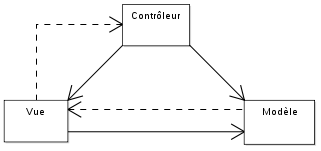
\includegraphics{ModeleMVC.png}
		\end{center}
	\caption{Notre adaptation du modèle MVC}
	\label{modeleMVC}
	\end{figure}

	Lorsque l'utilisateur interagit avec les boutons de l'interface ou avec
	l'espace de jeu, celui-ci envoie une requête à l'application.
	Cette requête est envoyée depuis la vue puis analysée par le contrôleur.
	Ensuite, le contrôleur demande au modèle d'effectuer les traitements
	nécessaire. Enfin, le contrôleur renvoie la vue adaptée.
	

	\subsection{Les règles mises en place}
		\label{regles}

	Les différentes règles mises en place sont :
	
	\begin{itemize}
		\item Contrairement au Go, le but premier est de faire une prise et non la
		possession de territoires~;
		\item Le suicide est interdit sauf s'il permet une prise~;
		\item Un pion ou un groupe de pions est pris lorsque celui-ci n'a plus de
		libertés~;
		\item Le jeu est fini lorsqu'un pion ou un groupe de pions est pris.\\
    \end{itemize}
    
    Ces règles ont été mises en places à l'aide de différentes classes
    permettant la gestion de groupe et de coup. Des méthodes ont aussi été
    développées afin de connaître les libertés de chaques groupes et de
    vérifier qu'il n'y ait pas de suicide.

	\subsection{Choix de l'algorithme d'I.A}
		\label{choix_alpha_beta}
	Pour ce jeu, nous avons choisi d'implémenter l'algorithme alpha-bêta. En
	effet, celui-ci est plus performant que l'algorithme min-max. Il donne les
	mêmes résultats au niveau de la stratégie mais est plus performant quant à la
	rapidité. Le gain produit par cette méthode est très important alors que les
	modifications à apporter à l'algorithme min-max sont simples.
	
	Dans un premier temps, nous avions envisagé de construire un arbre puis de
	l'évaluer. Cet arbre ne sera jamais supprimé mais évoluerais au cours de la
	partie. Cependant, cette méthode nécessitait trop de mémoire, c'est pourquoi
	nous l'avons abandonnée.
	
\clearpage		
\section{Interface Homme-Machine}
L'IHM n'est pas le plus important de ce projet, cependant une IHM
représente quand même une partie importante du développement d'un projet.
\subsection{L'interface de base}
Dans ce programme, l'IHM(Figure \ref{IHM_Vide}) est assez primaire avec une
barre de menu et le plateau de jeu :  le Goban.\\

	\begin{figure}[!ht]
    	\begin{center}
			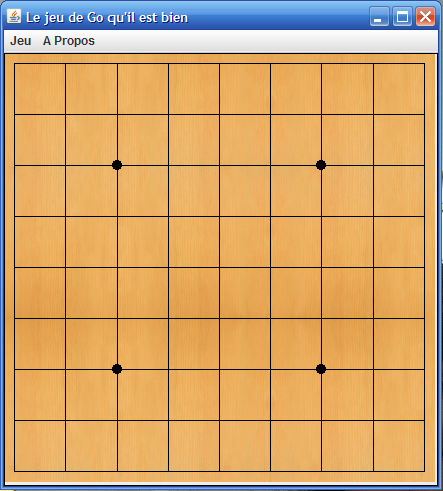
\includegraphics[scale=0.5]{IHM_Vide.png}
		\end{center}
	\caption{L'interface du programme}
	\label{IHM_Vide}
	\end{figure}

Cette IHM est constituée de deux parties comme le montre le diagramme de
classe(Figure \ref{diag_IHM}) :

	\begin{itemize}
  		\item Une partie correspondant au plateau de jeu~; 
		\item Une partie correspondant à la fenêtre de base(sans le Goban).\\
    \end{itemize}
    
    	\begin{figure}[!ht]
    	\begin{center}
			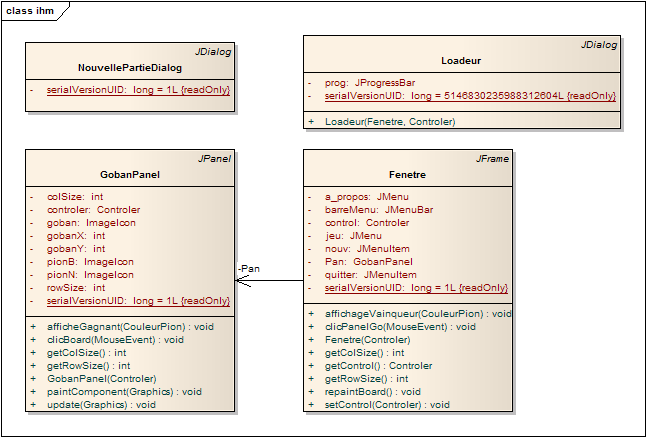
\includegraphics[scale=0.7]{diag_IHM.png}
		\end{center}
	\caption{Diagramme de classe de l'IHM}
	\label{diag_IHM}
	\end{figure}   
  

Les menus sont constitués d'un sous-menu permettant le démarrage d'une nouvelle
partie et un autre qui sert à quitter l'application. 

\subsection{Le déroulement du jeu}
Lors du démarrage d'une nouvelle partie, une boite de dialogue s'affiche
demandant à l'utilisateur le mode de jeu et la difficulté de l'intelligence artificielle.
Le mode de jeu correspond à un Atari-go entre deux joueurs ou entre un joueur
et un ordinateur. De plus, l'utilisateur peut définir le nombre de prise
déterminant l'arrêt du jeu.\\

Toutes les interactions avec le Goban sont envoyés au modèle afin que les
différentes méthodes assurant le respect des règles de jeu, présentées dans la
section \ref{regles} soit lancées. Une fois ceci assuré, la vue est
actualisée afin que le pion apparraissent sur le plateau de jeu.
Pendant le déroulement du jeu, chaque pion est affiché après vérification.

Lorsqu'une prise est effectuée, les pions pris disparaissent du plateau de jeu.
Une fenêtre popup apparait alors affichant la couleur du groupe gagnant.
Le goban est ensuite vidé afin de pouvoir démarrer une nouvelle partie.
\clearpage
\section{Intelligence Artificielle}
L'intelligence artificielle est la partie la plus importante de ce projet car
c'est celle-ci qui constitue le lien entre ce programme et le module.
Pour réaliser cette intelligence, nous nous sommes basés sur l'algorithme
alpha-bêta vu en cours. Les raisons de ce choix ont été annoncés dans la
section \ref{choix_alpha_beta}.

\subsection{Le développement de l'I.A}
Dans un premier temps, nous avons mis en place les différentes règles du jeu
présentées dans la section \ref{regles} afin de pouvoir jouer avec le mode
joueur contre joueur.

Une fois ceci réalisé, nous avons pu commencer à mettre en place l'intelligence
artificielle. Nous avons juste adapté les méthodes de notre modèle mises en
place pour les joueurs humains afin que l'I.A puisse les utiliser.\\

Un sous-package du modèle gère l'intelligence que nous avons développé. On peut
observer dans le diagramme de classe(Figure \ref{diag_intel}) de ce sous-package
les méthodes composant notre intelligence, comme par exemple la méthode
alpha-bêta représentant l'implémentation de l'algorithme homonyme. Pour cette
gestion, nous avons choisi d'utiliser cet algorithme permettant une
bonne efficacité et une bonne rapidité de réaction. Nous avons intégré une notion
de difficulté de jeu en relation avec la profondeur de l'arbre géré par cet
algorithme.

    \begin{figure}[!ht]
    	\begin{center}
			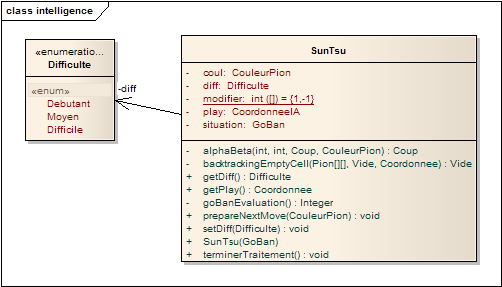
\includegraphics[scale=0.7]{diag_intel.png}
		\end{center}
	\caption{Diagramme de classe de l'I.A}
	\label{diag_intel}
	\end{figure} 

\subsection{L'heuristique}
	\label{heuristique}
Pour obtenir une bonne heuristique, nous avons pris en compte de nombreux
aspects du jeu. \\

Tout d'abord, nous avons observé que la situation de jeu
appellé "oeil" est importante.

Nous avons donc utilisé les "yeux" ainsi que des notions de jeu telles que la
perte de libertés, les groupes de pions, \dots{} pour faire une bonne
heuristique.

Pour repérer une situation correspondant à un "oeil", nous avons mis en place
un système de backtracking permettant la reconnaissance de zones vides les
constituant.\\

La difficulté dans le jeu d'Atari-Go est de favoriser la prise tout en se
protégeant de l'adversaire.

De plus, il ne faut pas tout le temps considérer la perte de libertés comme un
désavantage.
Pour notre heuristique, chaque situation est pondérée afin d'obtenir les
meilleurs résultats possibles.\\

La difficulté de notre intelligence est basée sur la profondeur de notre arbre
de calcul. Plus l'arbre est profond, plus l'intelligence artificielle est bonne.
Lorsque la difficulté choisie est facile, la profondeur de l'arbre est de 4. En
ce qui concerne les difficultés moyenne et difficile, les profondeurs sont
respectivement de 6 et 8.\\


\clearpage
\section{Difficultés rencontrées}
Tout d'abord, au niveau de l'interface, une des difficultés a été de mettre en
relation le pixel où le clic du joueur a été effectué et une intersection du
goban.\\

Ensuite, la plus grosse difficulté a été de déterminer une bonne heuristique.
En particulier pour le jeu d'Atari-Go, où de nombreuses situations de jeu sont
à prendre en compte.

L'algorithme qui permet la reconnaissance de situations, comme décrit dans la
section \ref{heuristique}, a été compliqué à mettre en place. En effet, cet
algorithme de reconnaissance devait être efficace, rapide et juste.\\

Enfin, un des problèmes posés a été de mettre en place la limite du temps de
reflexion de notre intelligence. Celle-ci a été effectué à l'aide de threads et
le fait d'interrompre l'algorithme alpha-bêta n'a pas été facile à gérer.
 \clearpage	
\section{Conclusion}
En conclusion, ce projet a été, pour nous, intéressant du point de vue
développement. En effet, il nous a permis de mettre en place une application
entière avec les complications que cela comporte. Cette application nous a
permis de voir aussi une implémentation concrète d'un algorithme d'intelligence
artificielle vu en cours. Le fait de faire un jeu a aussi été un attrait
supplémentaire.

\end{document}
